\documentclass[pdf,xcolor=dvipsnames,noparindent]{beamer}

\usetheme{Warsaw}
\usecolortheme{spruce}

% packages
\usepackage{listings}
% \usepackage{upquote}

% \lstset{numbers=left, numberstyle=\footnotesize, stepnumber=1,firstnumber=1,
%     numbersep=5pt,
%     stringstyle=5pt,
%     basicstyle=\footnotesize,
%     keepspaces=true, tabsize=4,
%     showstringspaces=false
%     % backgroundcolor=\color{SpringGreen}
% }

% preamble
\title{Introduction to Go - Part 1}
\author{Wojciech Gac}
\date{July 26, 2019}

% document proper
\begin{document}

\begin{frame}
	\titlepage
\end{frame}

% \begin{frame}{Outline}
% 	\pause
% 	\begin{itemize}
% 		\item The Problem
% 		      \pause
% 		\item Delve Debugger
% 		      \pause
% 		\item Container Preparation
% 		      \pause
% 		\item Debugging
% 		      \pause
% 		\item Further Reading
% 	\end{itemize}
% \end{frame}

% \begin{frame}
% 	\frametitle{The Problem}
% 	We'd like to be able to do the following:
% 	\pause
% 	\begin{itemize}
% 		\item Using a local instance of VSCode...
% 		      \pause
% 		\item ...and a dockerized instance of a Go application...
% 		      \pause
% 		\item ...connect to a running process \emph{inside} the container...
% 		      \pause
% 		\item ...interrupt execution with breakpoints and modify variables on the fly
% 	\end{itemize}
	  
% \end{frame}

\begin{frame}{Outline}
  \pause
  \begin{itemize}
  \item Origins of Go
    \pause
  \item Language Basics
    \pause
  \item Concurrency Patterns
    \pause
  \item Practical Use Cases
    \pause
  \end{itemize}
\end{frame}

\begin{frame}{Origins of Go}
  \pause
  \begin{itemize}
  \item Designed at Google in 2007
    \pause
  \item ... by Rob Pike, Ken Thompson and Robert Griesemer
    \pause
  \item ... two of whom (Pike \& Thompson) had spent decates at Bell Labs
    \pause
  \item ... building on a long history of concurrent languages
    \pause
  \item ... such as Occam, Erlang, Newsqueak, Concurrent ML, Alef and Limbo
  \end{itemize}
  
\end{frame}

\begin{frame}{Origins of Go}
  \pause
  \begin{itemize}
  \item Heavily influenced by Tony Hoare's CSP paper from 1978
    \begin{figure}
      \centering
      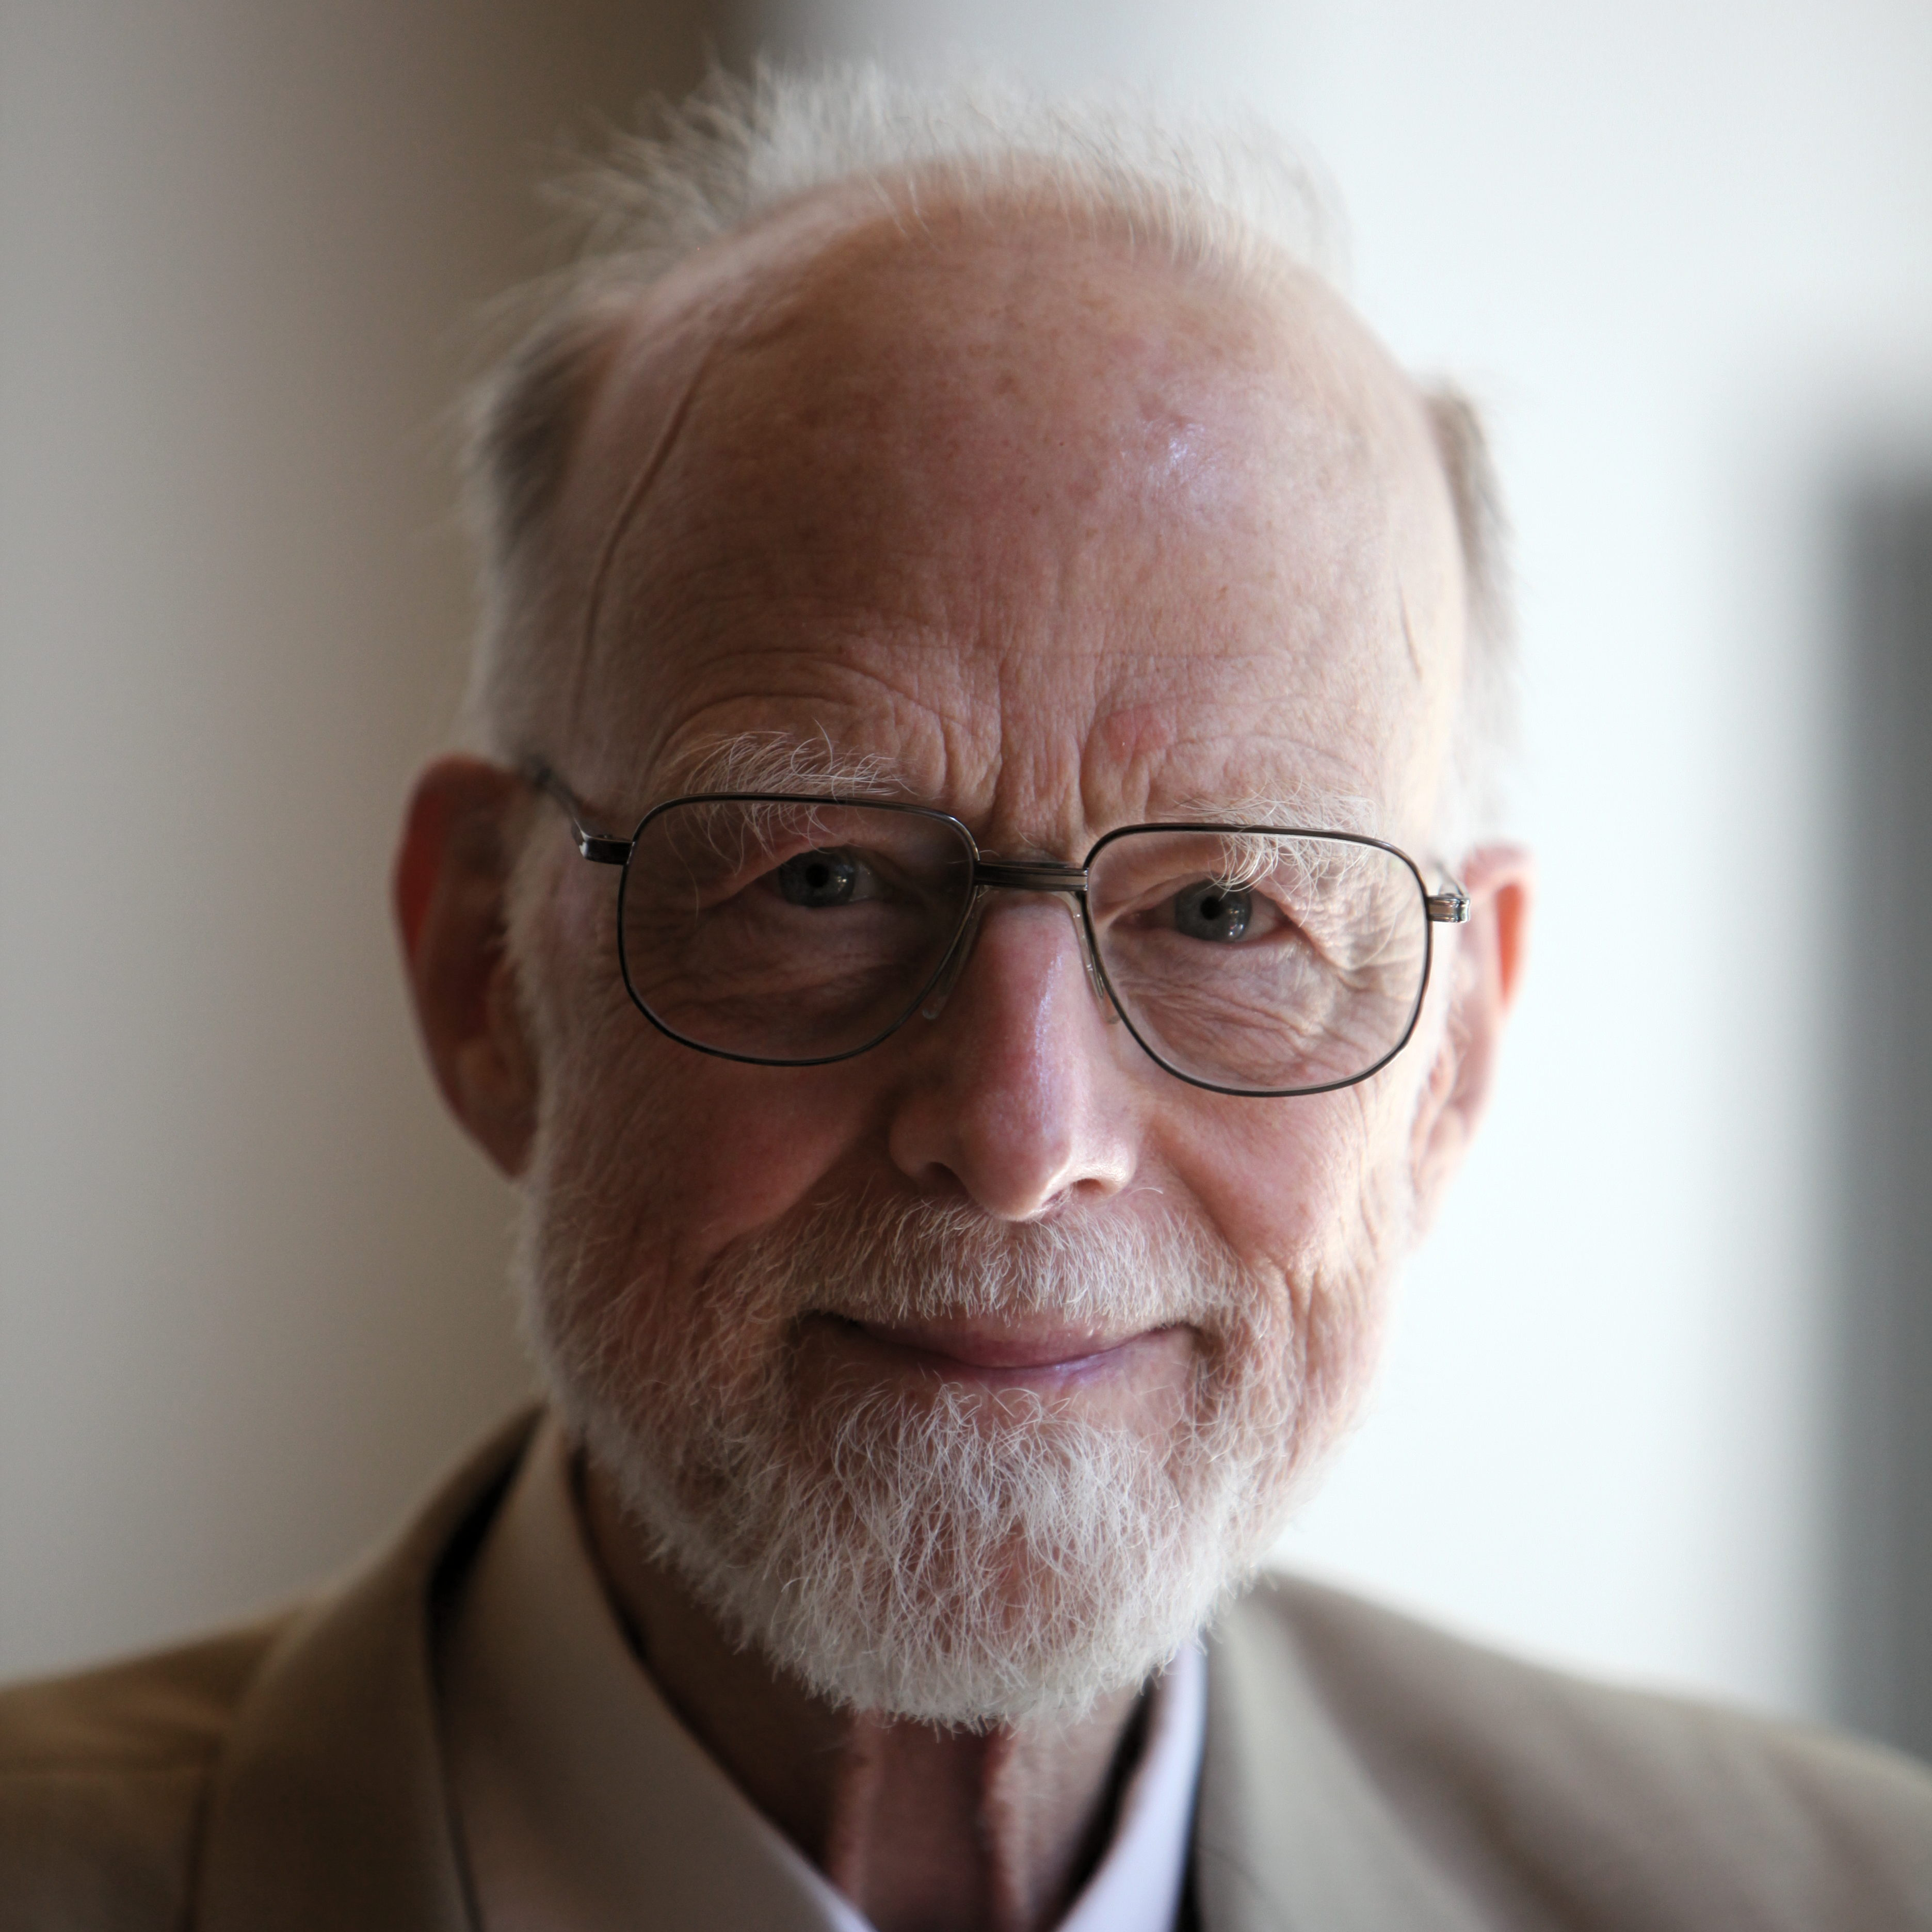
\includegraphics[scale = 0.02]{images/hoare.jpg}
    \end{figure}
    \pause
  \item ... in which input and output operations are programming primitives
    \pause
  \item ... helping structure parallel process communication
  \end{itemize}
  
\end{frame}

\begin{frame}{Origins of Go}
  \pause
  Rationale:
  \pause
  \begin{itemize}
  \item C++ compile cycles took too long at Google
    \pause
  \item The C model was efficient, but lacked more modern facilities \& libraries
    \pause
  \item A fast, compiled, no-nonsense systems programming language was needed
    \pause
  \item Memory safety, garbage collection, structural typing and concurrency were prioritized
    \pause
  \item Module/namespace system facilitated development of very large systems without name collisions
    \pause
  \item Good style had to be formalized to avoid ambiguity
  \end{itemize}
\end{frame}

\begin{frame}{Origins of Go}
  \pause
  Things happen fast...\\
  \pause
  ...when you're backed by Google
\end{frame}

\begin{frame}{Origins of Go}
  \pause
  A (very) incomplete list of adopters:
  \begin{itemize}
  \item Docker
    \pause
  \item Dropbox
    \pause
  \item Uber
    \pause
  \item Cloud Foundry
    \pause
  \item Ethereum
    \pause
  \item Netflix
    \pause
  \item Heroku
    \pause
  \item MongoDB
    \pause
  \item Allegro
    \pause
  \item OLX
    \pause
  \item Yandex.ru
    \pause
  \item Google - obviously
  \end{itemize}
\end{frame}

\begin{frame}{Language Basics}
  \pause
  Language attributes:
  \begin{itemize}
    \pause
  \item Compiled to native code
    \pause
  \item Garbage collection
    \pause
  \item Statically typed
    \pause
  \item Syntax similar to C
    \pause
  \item Rich default toolchain
    \pause
  \item Official formatting style (enforced by the compiler)
    \pause
  \item Simplified model of OOP (structs, methods, interfaces)
  \end{itemize}
\end{frame}

\begin{frame}[fragile]{Language Basics}
  \pause
  Variables:
  \pause
  \begin{itemize}
  \item Variable declaration:
    \begin{semiverbatim}
      var <name> <type>
    \end{semiverbatim}
    \pause
  \item Variable assignment:
    \begin{semiverbatim}
      <name> = <value>
    \end{semiverbatim}
    \pause
  \item Combined declaration \& assignment:
    \begin{semiverbatim}
      var <name> <type> = <value>
    \end{semiverbatim}
    \pause
  \item Short declaration with type inference (a'la C++ \texttt{auto}):
    \begin{semiverbatim}
      <name> := <value>
    \end{semiverbatim}
  \end{itemize}
\end{frame}

\begin{frame}{Language Basics}
  \pause
  Basic data types:
  \pause
  \begin{itemize}
    \begin{columns}
      \column{0.4\textwidth}
    \item \texttt{int}
    \item \texttt{int8}
    \item \texttt{int16}
    \item \texttt{int32}
    \item \texttt{int64}
      \pause
    \item \texttt{uint}
    \item \texttt{uint8}
    \item \texttt{uint16}
    \item \texttt{uint32}
    \item \texttt{uint64}
    \item \texttt{uintptr}
      \pause
      \column{0.4\textwidth}
    \item \texttt{bool}
      \pause
    \item \texttt{string}
      \pause
    \item \texttt{byte}
    \item \texttt{rune}
      \pause
    \item \texttt{float32}
    \item \texttt{float64}
      \pause
    \item \texttt{complex64}
    \item \texttt{complex128}
      \end{columns}
  \end{itemize}
\end{frame}

\begin{frame}[fragile]{Language Basics}
  \pause
  Function definitions:
  \pause
  \begin{semiverbatim}
    func <name>(<parameters>...) <return-types>... \{
      // body... 
      
      // optional
      return <return-value>
    \}
  \end{semiverbatim}
\end{frame}

\end{document}